% !TeX spellcheck = en_US
\documentclass{beamer}
\usepackage[latin1]{inputenc}
\usepackage{dsfont}
\usepackage{color}
\usepackage{tabularx}
\usepackage{amssymb}
\usepackage{verbatim}
\usepackage{booktabs}
\usepackage{tikz}
\usetikzlibrary{arrows}

% % % % % FRAME STYLE

% NEW
%\usetheme{Frankfurt}
%\setbeamertemplate{navigation symbols}{}
%\setbeamertemplate{frametitle}[default][center]

% OLD
\setbeamertemplate{navigation symbols}{}
\setbeamertemplate{frametitle}{\vspace{5mm}\hspace{0mm}\insertframetitle}
%\setbeamertemplate{frametitle}[default][center]
\setbeamertemplate{footline}{\hfill\insertframenumber/\inserttotalframenumber\hspace{5mm}\vspace{5mm}}
\AtBeginSection[]
{
	\begin{frame}
		\frametitle{Agenda}
		\tableofcontents[currentsection]
	\end{frame}
}

\usefonttheme{structurebold}
\usecolortheme{dove}

% % % % % CUSTOM COMMANDS
\newcommand{\Empty}{\mbox{$\varnothing$}}
\newcommand{\NotEmpty}{\mbox{$\neg\varnothing$}}
\newcommand{\ToDo}{\textcolor{red}{TODO}}
\newcommand{\Highlight}[1]{\textcolor{purple}{#1}}
% % % % % FRAMES

\begin{document}

	\title{Qualitative Spatial Reasoning over Line-Region Relations}
	\author{Leena and Sibel}
	\date{Knowledge Representation\\Seminar Presentation}
	
	\begin{frame}
		\titlepage
	\end{frame}
	
	\section{Motivation}
	% !TeX spellcheck = en_US

%TODO Leena

\begin{frame}{Motivation}
	\begin{itemize}
		\item Modeling spatial relations
		%\item \Highlight{\textbf{2}} geometrically distinct placements of the line for each of the \Highlight{\textbf{19}} topologically distinct relations \Highlight{$\implies$}
		
		\item How do humans conceptualize spatial relations?
		
		\item Strong correlation between Perceptual space and Language Space
		
		\item Understanding how language structures space

	\end{itemize}
\end{frame}


	
	\section{9-Intersection}	
	% !TeX spellcheck = en_US

%TODO Leena

\begin{frame}{9-Intersection}
	\begin{block}{Goal} 
	A computational model to describe conceptual neighborhoods and enable the definition of a similarity metric for line region relations.
		\end{block}
	\begin{block}{Conceptual Similarity: Which pairs of relationships are similar?}
	\begin{figure}
	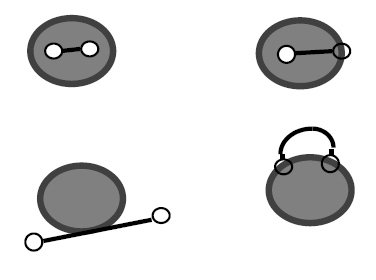
\includegraphics[width = 0.5\textwidth]{images/conceptualsimilarity.png}
	\end{figure}
\end{block}			
\end{frame}

\begin{frame}{Formal Definitions}
	\begin{block}{Line}
	A sequence of 1...n connected 1-cells between two geometrically independent 0-cells such that they neither cross each other nor form cycles.
	\begin{itemize}
	\item Interior, Boundary, Exterior
	\end{itemize}
\end{block}		
		\begin{figure}
		
\includegraphics[width=0.7\textwidth]{images/line.png}
\end{figure}
\end{frame}

\begin{frame}{Formal Definitions(contd.,)}
	\begin{block}{Region}
	A region is defined as a connected, homogeneously 2-dimensional 2-cell. Its boundary forms a Jordan curve separating the region's exterior from its interior.
	\begin{itemize}
	\item Interior, Boundary, Exterior
	\end{itemize}
\end{block}		
		\begin{figure}
		
\includegraphics[width=0.7\textwidth]{images/region.png}
\end{figure}
\end{frame}

\begin{frame}{Adjacency}
	\begin{block}{Topological adjacency}
	\begin{itemize}
	\item Adjacent(Interior {$A^0$}) = $\partial A$
	\item Adjacent(Boundary {$\partial A$}) = $A^0 and A^-$
	\item Adjacent(Exterior {$A^-$}) = $\partial A$
	\end{itemize}
\end{block}		
\end{frame}

\begin{frame}{9-Intersection(contd..,)}
	\begin{block}{Topological adjacency}
	\begin{itemize}
	\item 9 intersections between the different topological parts of a line and a region
	\end{itemize}
\end{block}		
\begin{block}{The 9-intersection Matrix(M)}
\[ \left( \begin{array}{ccc}
L^0 \cap R^0  & L^0 \cap \partial R & L^0 \cap R^- \\
\partial L \cap R^0 & \partial L \cap \partial R & \partial L \cap R^- \\
L^- \cap R^0 & L^- \cap \partial R & L^- \cap R^- \end{array} \right)\] 
\end{block}
\end{frame}

\begin{frame}{9-Intersection(contd..,)}
	\begin{block}{}
	\begin{itemize}
	\item Binary assignment to intersections($\emptyset,  -\emptyset$)
	\item \textbf{512} possible instances of M
	\item \textbf{19} of 512 instances can actually be realized.
	\end{itemize}
\end{block}		
\begin{block}{Example}
\begin{figure}[l]
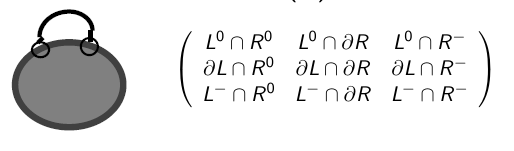
\includegraphics[width = \textwidth]{images/9examplemat.png}
\end{figure} 
\end{block}
\end{frame}

\begin{frame}{9-Intersection(contd..,)}
	\begin{block}{}
	\begin{itemize}
	\item Binary assignment to intersections($\emptyset,  -\emptyset$)
	\item \textbf{512} possible instances of M
	\item \textbf{19} of 512 instances can actually be realized.
	\end{itemize}
\end{block}		
\begin{block}{Example}
\begin{figure}[l]
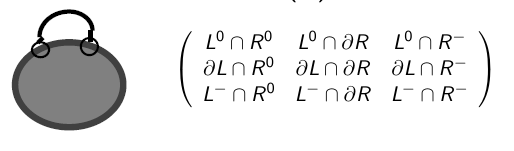
\includegraphics[width = \textwidth]{images/9examplemat.png}
\end{figure} 
Compute the values of the matrix...
\end{block}
\end{frame}


\begin{frame}{Geometric interpretations}	
\begin{figure}[l]
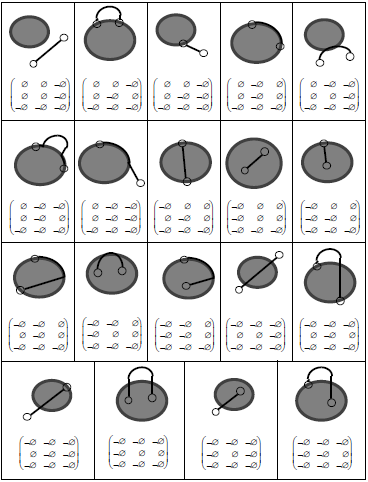
\includegraphics[width = 0.55\textwidth]{images/9intersection.png}
\end{figure} 
\end{frame}


	
	\section{Snapshot Model}	
	% !TeX spellcheck = en_US

%TODO Leena

\begin{frame}{Snapshot Model}
\begin{itemize}
\item A model of conceptual neighborhood among topological relations between a line and a region.
\end{itemize}

		\begin{block}{Characteristics}
	\begin{itemize}
	
	\item No prior knowledge of the potential transformations that could lead from one configuration to the other. 
	\item Comparison on the basis of a pre-defined distance metric  
	\end{itemize}
	
		\end{block}
		
		\begin{block}{Differences of Intersections(\Empty = 0, \NotEmpty = 1)}
		\begin{figure}
		\begin{center}
			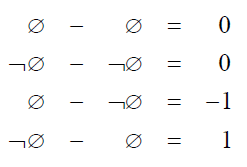
\includegraphics[width = 0.4\textwidth]{images/snapshotdiff.png}
		\end{center}
		\end{figure}
		\end{block}
	\end{frame}
	
	\section{Smooth-Transition Model}	
	% !TeX spellcheck = en_US

%TODO Sibel

\begin{comment}
	- second conceptual neighborhood model
	- smooth transition: definition
	- occurrence of smooth transition -> conceptual neighborhood
	\end{comment}

	\begin{frame}{Smooth-Transition Model}
		\begin{block}{Example}
			A pair of line-region relations that are conceptual neighbors (one can be obtained from the other via a ''smooth transition'')
		\end{block}
		
		\begin{block}{Counterexample}
			A pair of line-region relations that \textbf{not} are conceptual neighbors
		\end{block}
	\end{frame}
	
	\begin{frame}{Formalization}
		\begin{block}{Possible Changes} A smooth transition can occur by:
			\begin{itemize}
				\item Moving around a line's boundary nodes
				\begin{itemize}
					\item[Rule 1] Line's two boundary nodes intersect with same region part
					\item[Rule 2] Line's two boundary nodes intersect with different region part
				\end{itemize}
				\item Moving around a line's interior
				\begin{enumerate}
					\item[Rule 3] Extend line's interior-intersection partially
					\item[Rule 4] Reduce line's interior-intersection partially
				\end{enumerate}
			\end{itemize}
		\end{block}
		
%		In terms of 9-Intersection, a smooth transition means that an intersection or its adjacent intersection gets changed from empty to non-empty, or reverse.
	\end{frame}
	
	\begin{frame}{Extent of a Line Part}
		Extent of a part $i$: Denoted by $ \#M[i, \_]$; number of non-empty intersections between $i$ and th three parts of the second object.
		Define extent of a part i Draw 9-intersection model on the board for reference
		
		\begin{itemize}
			\item (Explain on the board) The extent of a line's interior with respect to a region is in the interval of 1 to 3, the extent of the lines boundary is either 1 (if both nodes are located in the same region part) or 2 (if the nodes are located in different parts of the region), and the extent of a line's interior is always 3.
		\end{itemize}
	\end{frame}
	
%	\begin{frame}{First Rule}
%		If the line's two boundaries intersect with the same region part, then extend the intersection to either of the adjacent region parts.
%		\begin{block}{Formalization}
%			\centering $ \#M[\delta, \_] = 1 \Rightarrow
%			\forall i (M[\delta, i] = \NotEmpty):
%			M_{N}[\delta, \text{adjacent}(i)] := \NotEmpty $
%		\end{block}
%		
%		\begin{block}{Example}
%			%Moving one boundary of a line into an adjacent part of the region.
%			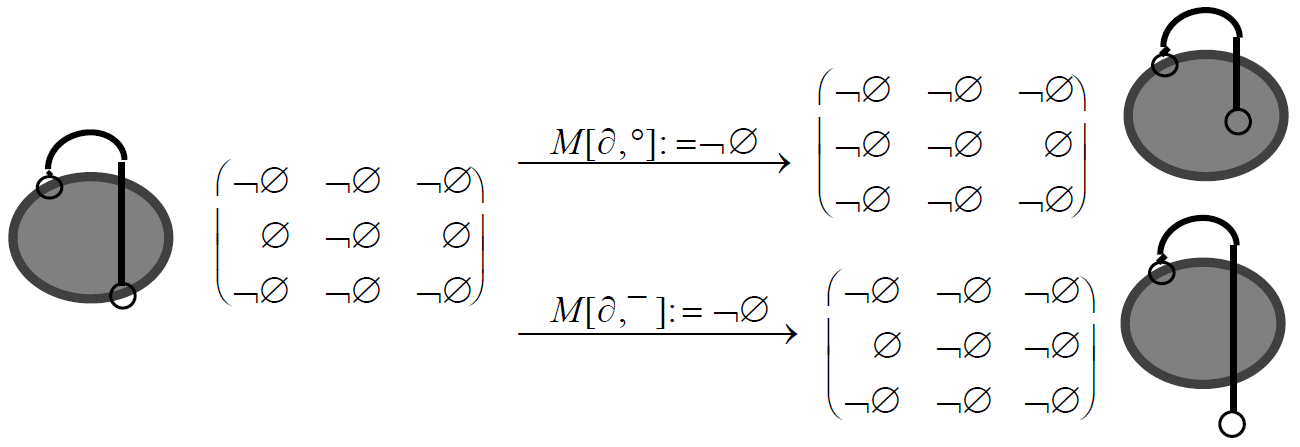
\includegraphics[width=\textwidth]{images/smooth_transitions_example_a.png}
%		\end{block}
%	\end{frame}
%	
%	\begin{frame}{Second Rule}
%		If the line's two boundaries intersect with two different region parts then move either intersection to the adjacent region part.
%		\begin{block}{Formalization}
%			\centering $ \#M[\delta,\_] = 2 \Rightarrow
%			\forall i (M[\delta, i] = \NotEmpty):
%			M_{N}[\delta, i] := \Empty \text{ \textbf{and} }
%			M_{N}[\delta, \text{adjacent}(i)] := \NotEmpty $
%		\end{block}
%		
%		\begin{block}{Example}
%			%Moving either boundary into an adjacent region part.
%			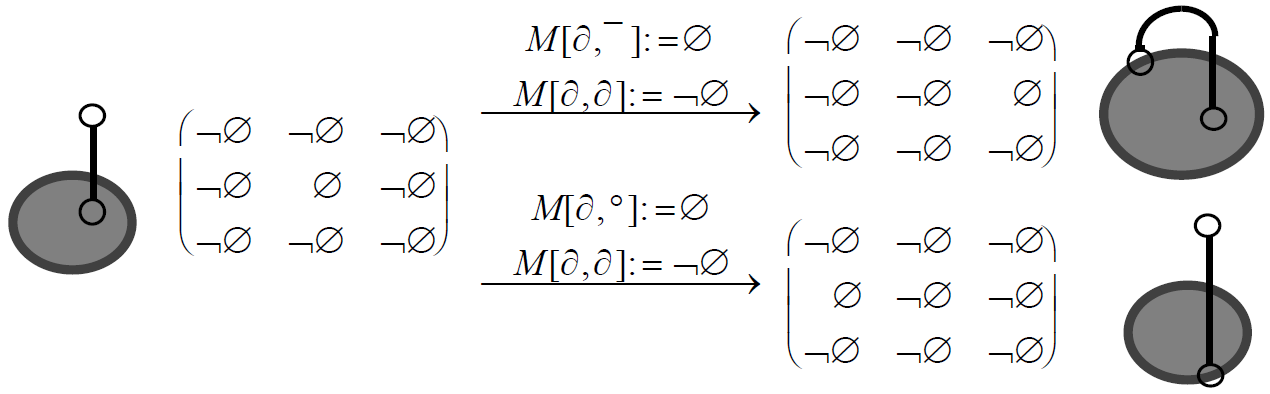
\includegraphics[width=\textwidth]{images/smooth_transitions_example_b.png}
%		\end{block}
%	\end{frame}
%	
%	\begin{frame}{Third Rule}
%		Extend the line's interior-intersection to either of the adjacent region parts.
%		
%		\begin{block}{Formalization}
%			\centering $ \forall i (M[°, i] = \NotEmpty):
%			M_{N}[°, \text{adjacent}(i)] := \NotEmpty $
%		\end{block}
%		
%		\begin{block}{Example}
%			%Moving the line's interior into an adjacent part of the region.
%			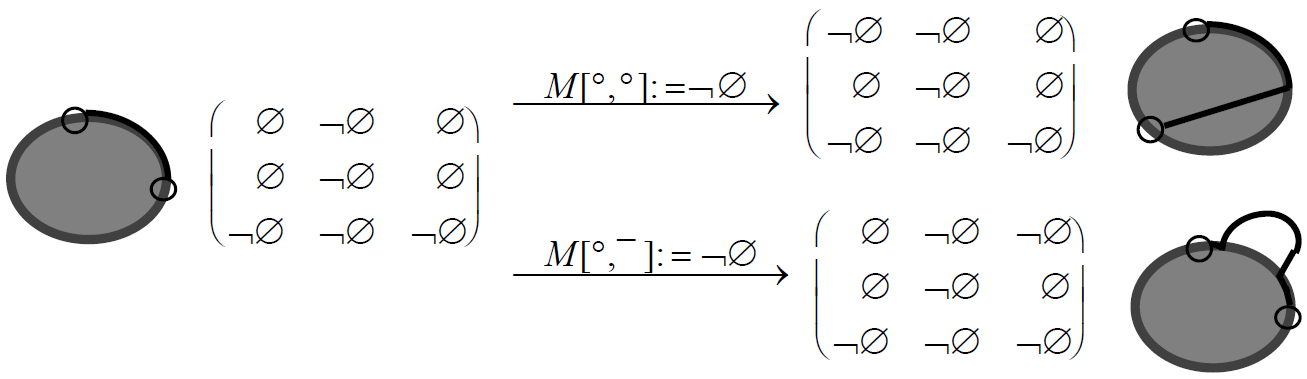
\includegraphics[width=\textwidth]{images/smooth_transitions_example_c.png}
%		\end{block}
%	\end{frame}
%	
%	\begin{frame}{Fourth Rule}
%		Reduce the line's interior intersection on either of the adjacent region parts.
%		
%		\begin{block}{Formalization}
%			\centering
%			$ \#M[°, \_] = 2 \Rightarrow
%			\forall i (M[°, i] = \NotEmpty):
%			M_{N}[°, i] := \Empty $
%			$ \#M[°, \_] = 3 \Rightarrow
%			\forall i (i \neq \delta):
%			M_{N}[°, i] := \Empty $
%		\end{block}
%		
%		\begin{block}{Example}
%			%Moving the line's interior out of a part of the region.
%			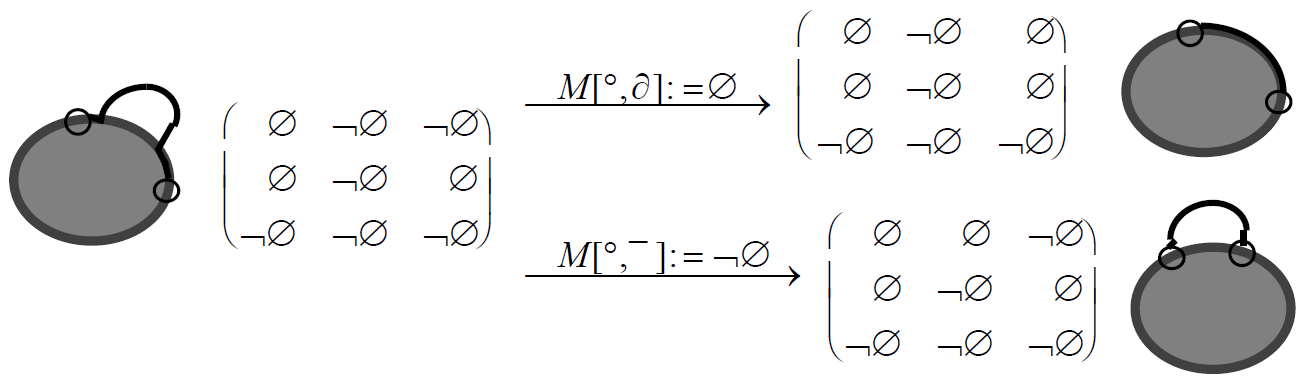
\includegraphics[width=\textwidth]{images/smooth_transitions_example_d.png}
%		\end{block}
%	\end{frame}
%	
%	\begin{frame}{Consistency Constraints}
%		\begin{enumerate}
%			\item If the line's interior intersects with the region's interior \textit{and} exterior, then the line's interior must also intersect with the region's boundary.
%			\begin{center}
%				$ M[°,°] = \NotEmpty \text{and} M[°,^{-}] = \NotEmpty \Rightarrow M[°,\delta] := \NotEmpty $
%			\end{center}
%			
%			\item If the line's boundary intersects with the region's interior (exterior) then the line's interior must intersect with the region's interior (exterior) as well.
%			\begin{center}
%				$ M[\delta, °] = \NotEmpty M[°,°] := \NotEmpty $ \\
%				$ M[\delta, ^{-}] = \NotEmpty M[°,^{-}] := \NotEmpty $
%			\end{center}
%		\end{enumerate}
%		
%	\end{frame}
	
	% NOTES:
	% The separate moves of the line's interior and boundaries are atomic operations that do not account for some of the properties of the objects and their embedding space and, therefore, may generate inconsistent 9-intersections for configurations that cannot be realized. In order to maintain connectivity among the line's boundaries and interior, it is necessary to assure the following \textbf{consistency constraint}: [1]. Likewise, in order to preserve the continuous-space property of $\mathcal{R}^{2}$, the following consistency constraint must be fulfilled: [2].
	
	\begin{frame}{Resulting Neighborhood Graph}
		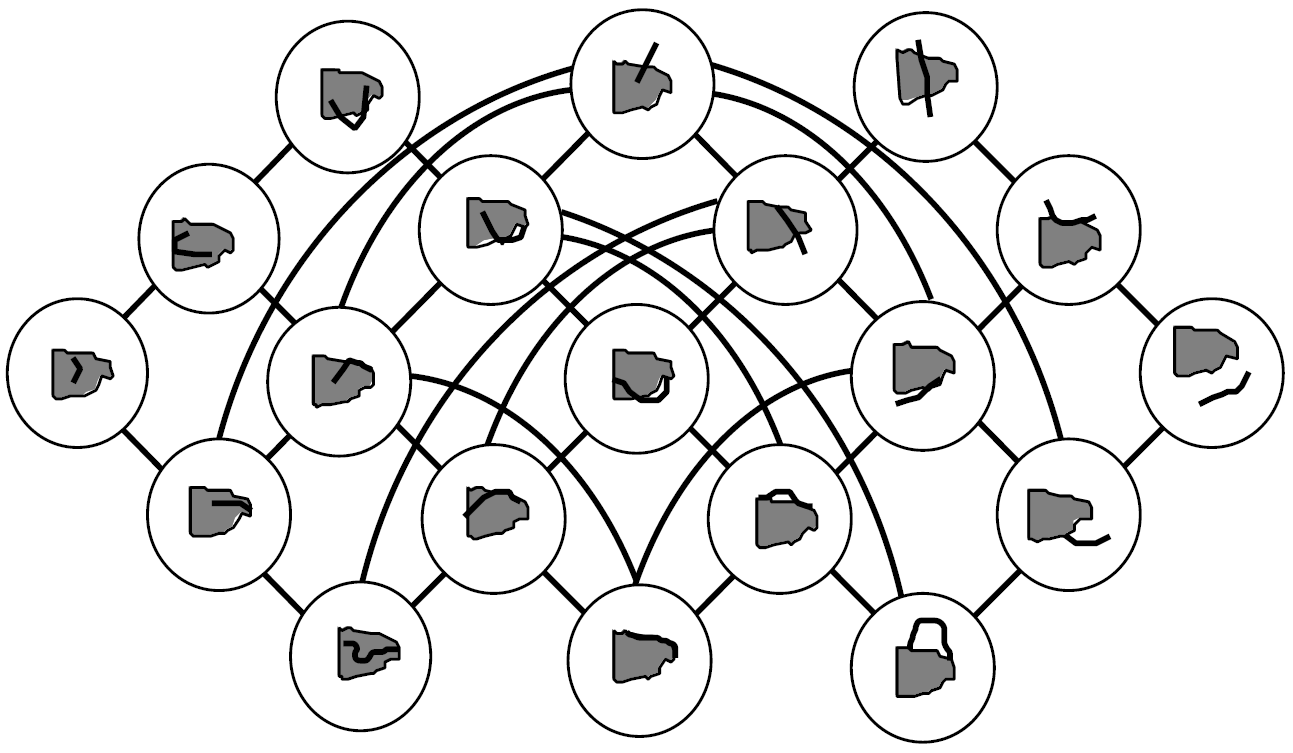
\includegraphics[width=\textwidth]{images/smooth_transitions_neighborhood_graph.png}
	\end{frame}
	
	\begin{comment}
		- images are a bit small
		- the purpose is to give the audience just a feeling of how similar/ different the models are
		- resemble a lot in structure
		- differences are the way in which conceptual neighbors are connected at the to and the additional links that run across the smooth transition graph
	\end{comment}
	
	\begin{frame}{Juxtaposition of Neighborhood Graphs}
		\begin{tabularx}{\textwidth}{XX}
			\begin{center}
				\textbf{Snapshot Model}
			\end{center}
			&
			\begin{center}
			\textbf{Smooth-Transition Model}
			\end{center} \\
			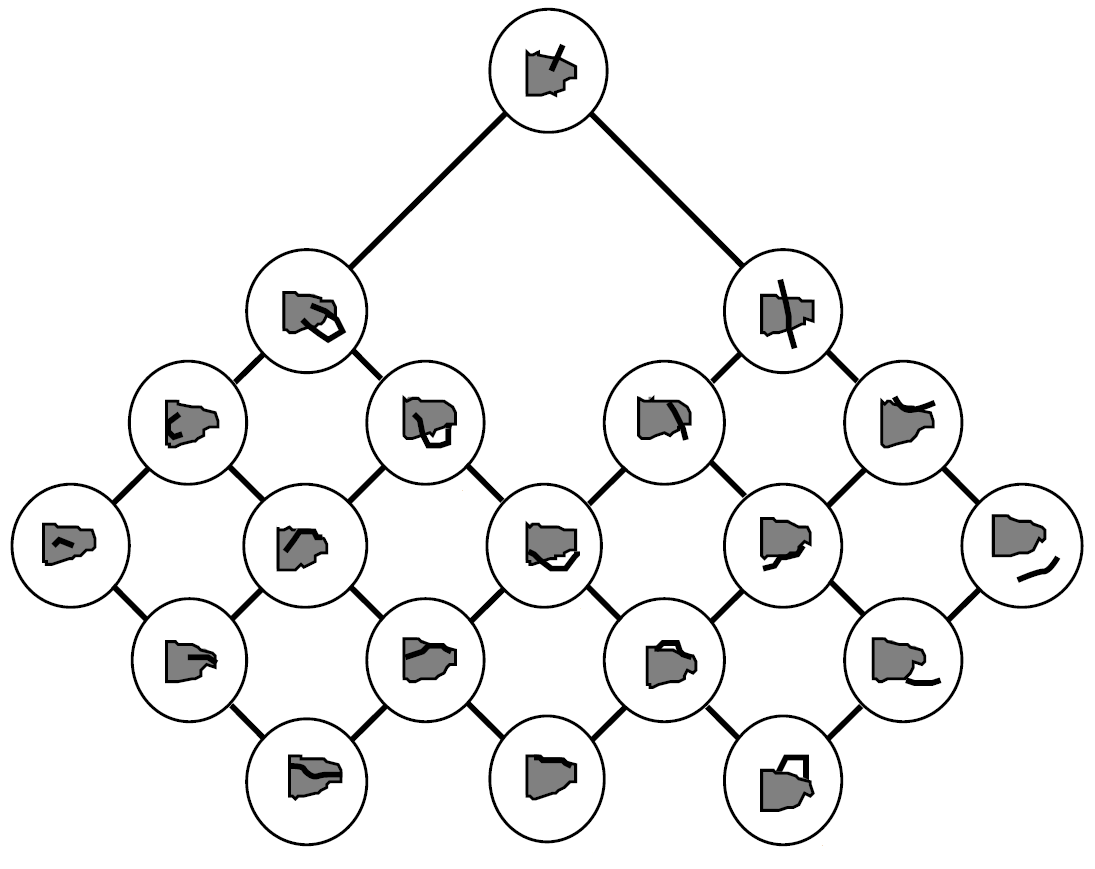
\includegraphics[width=0.48\textwidth]{images/snapshot_model_neighborhood_graph_simple.png}
			&
			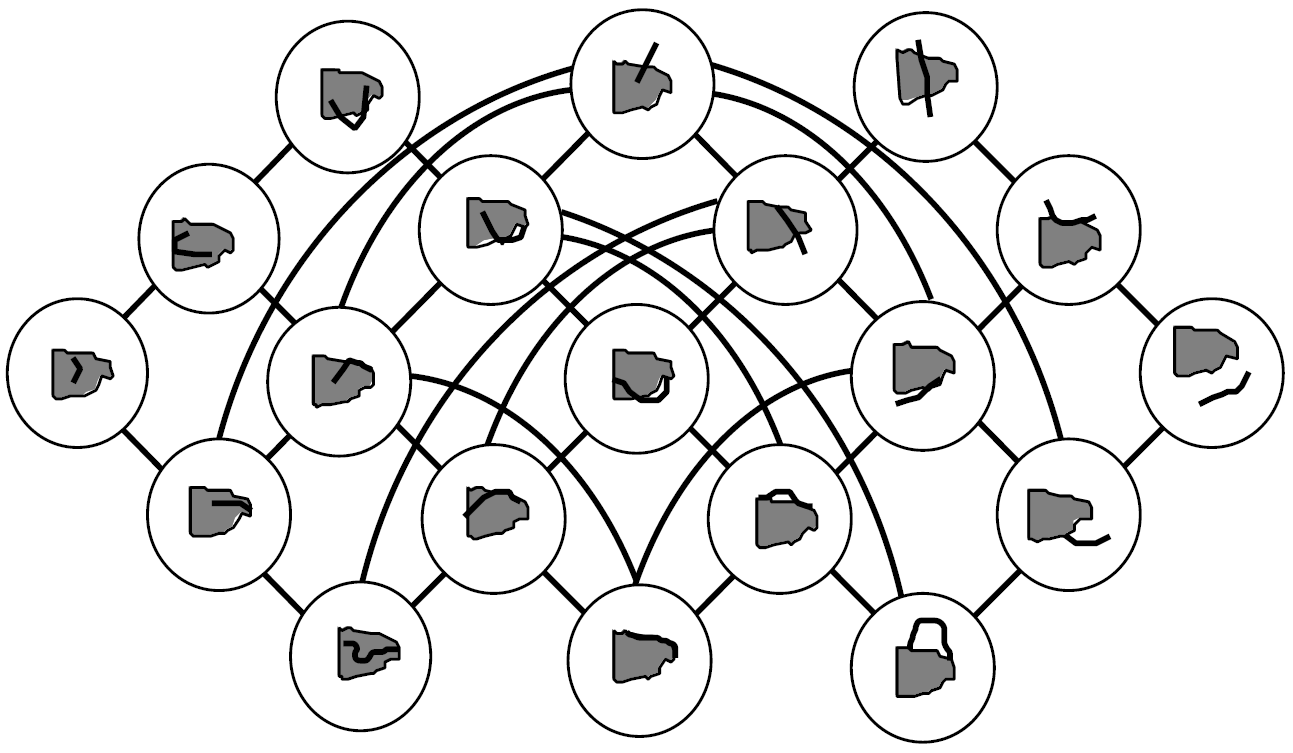
\includegraphics[width=0.48\textwidth]{images/smooth_transitions_neighborhood_graph.png}
		\end{tabularx}
	\end{frame}
	
	\begin{comment}
		\begin{itemize}
		\item 19 line-region relations $\rightarrow$ 171 distinct pairs of relations that can possibly be conceptual neighbors
		\item 26 under snapshot model and the smooth-transition model
		\item 2 under snapshot model
		\item 12 under smooth-transition model
		\item 131 pairs under neither model
		\end{itemize}
	\end{comment}	
	
	\section{Evaluation}	
	% !TeX spellcheck = en_US

%TODO Sibel

\begin{frame}{Experiment}
	\begin{itemize}
		\item reused data from previous human-subject experiments
		\item GOAL: Within the context of different models for conceptual neighbors, it is particularly enlightening to analyse how the subjects formed groups of similar relations.
		
		\item group spatial relations between line and region, road and park (parks were all the same size and shape)
		\item 28 subjects performing tasks
		\item 38 diagrams % each of which showed a line and a region, said to be a road and a park respectively
		2 geometrically distinct placements of the road corresponding to each of the 19 topologically distinct relations
		\ToDo Example from Mark1994
		\item each spatial relation could be grouped as many as 112 times (4 pairs times 28 subjects) with each other relation
	\end{itemize}
	% As a basis for comparison, the pairs within each relation distinguished by the 9-intersection were grouped by all 28 subjects for 7 of the 19 relations, and by at least 23 subjects (82 per cent) for every relation. The maximum number of times that the stimuli in two different spatial relations were paired was 78 out of a maximum of 112 times (70 per cent).
\end{frame}

\begin{frame}{Participants}
\end{frame}

\begin{frame}{Results}
	\begin{itemize}
		\item The pairs that were neighbors by both snapshot and smooth-transition models were grouped from 0 to 78 times, with a mean of 33.6.
		
		\item Those pairs that were neighbors for smooth transitions-but not snapshots- were grouped between 0 and 66 times, with a mean of 17.3 (15.4 per cent).
		
		\item The two pairs that were snapshot neighbors-but not smooth transition neighbors- were grouped 10 and 16 times (mean = 14; 11.6 per cent).
		
		\item Perhaps most significant, however, is the fact that the 131 pairs that were neighbors by neither the snapshot model nor the smooth transitions were grouped an average of only 6.0 times by the subject (5.3 per cent of the maximum).
		
		\item Sixty pairs were never grouped by any of the 28 subjects nor any of the four possible stimulus pairs. The most frequently-grouped pair in this category was 54 times (48 per cent), but only 20 stimulus pairs with neither smooth transitions nor minimum snapshot difference were grouped 12 or more times (10 per cent of the maximum).
		
		\item 
	\end{itemize}
	
\end{frame}
	
	\section{Summary}
	% !TeX spellcheck = en_US

\begin{frame}{Summary}
	\begin{block}{ Two Conceptual Neighborhood Models}
		% based on the 9-intersection for binary topological relations, two models of conceptual neighborhoods among topological relations between a line and a region are developed
		
		% introduced two models for the similarity of topological line-region relations (snapshot model + smooth-transition model)
		
		\begin{enumerate}
			\item Snapshot Model
			% derives the neighborhoods by comparing pairs of topological relations and selects neighbors based on least noticeable differences
			
			\item Smooth-Transition Model
			%the smooth-transition model develops neighborhoods based on the knowledge of the deformations that may change a topological relation
		\end{enumerate}
		\textcolor{purple}{\textbf{Finding:}} \textit{Almost} identical Conceptual-Neighborhood Graphs
		% resulting similarity diagrams show some (minor) differences
	\end{block}
	\vspace{6pt}
	\begin{block}{Human-Subject Experiment}
		% tests in which human subjects were asked to organize line-region relations into groups of similar relations
		\textcolor{purple}{\textbf{Findings:}}
		\begin{itemize}
			\item confirmed that the conceptual neighborhoods identified by the two models correspond largely to the way humans conceptualize similarity about spatial relations
			\item \textbf{Finding:} groupings the subjects made indicate that the smooth-transition model captures more important aspects of the similarity of topological line-region relations than the snapshot model
			
			\item the majority of conceptual neighbors is the same in both diagrams, we conclude that the knowledge of a change process can be generally neglected when only considering topological similarity.
		\end{itemize}
	\end{block}
\end{frame}

\begin{comment}
The smooth-transition model represented the change process explicitly, whereas the snapshot model inferred change from topological differences.
\end{comment}
	
	\begin{comment}
		- citing style chicago
		- sorted by relevance
	\end{comment}
	\begin{frame}{References}
		\begin{itemize}
			\item Egenhofer, Max J., and David M. Mark. "Modelling conceptual neighbourhoods of topological line-region relations." \textit{International journal of geographical information systems 9}, no. 5 (1995): 555-565.
			
			\item Mark, David M., and Max J. Egenhofer. "Modeling spatial relations between lines and regions: combining formal mathematical models and human subjects testing." \textit{Cartography and geographic information systems 21}, no. 4 (1994): 195-212.
		\end{itemize}
	\end{frame}
	
\end{document}